\section{Value-based RL: Tabular Methods}
\textit{This section reviews the lecture slides 2 (Monte Carlo), 3 and 4.}
\subsection{Monte Carlo}
\begin{itemize}
	\item We can try to estimate the value function by simply sampling from the expectation, meaning we generate episodes, and evaluate the cumulative reward:
	$$v(s_t)=\E_{\pi}\left[\sum_{k=0}^{\infty} \gamma^k R_{t+k+1}\Big\vert S_t=s\right]\approx \frac{1}{N}\sum_{n=1}^{N}\sum_{k=0}^{T_{n}}\gamma^k R_{t+k+1}^{(n)}$$
	Note that this requires the task to be \textbf{episodic}, meaning that an episode always ends. Otherwise, we are not able to sample 
	\item We can get into the situation that we visit the same state twice in a trajectory. In the update, we can either just take the first time into account that we visited $s$ (\textit{first-visit MC}), or we can consider all of them as different points (\textit{every-visit MC}). Both approaches are very similar, and converge to the same optimum. However, every-visit MC leads to slightly biased estimates if number of samples is low.
	\item If we want to use Monte-Carlo for learning the optimal policy, we need to slightly adjust our algorithm. First, note that we rather want to learn the $q$-value as we can determine the optimal policy from them by greedifying: $\pi_{*}(s)=\arg\max_a q_{*}(s,a)$
	\item To guarantee that every state-action pair is visited, we can either:
	\begin{itemize}
		\item Perform ``exploring starts'', meaning that we randomly sample our start state $(S_0,A_0)$. However, note that this requires an environment where we can set the agent to any position, which is not always possible (e.g. in physical systems, hard to initialize velocity or acceleration)
		\item Use policy that visits every state and actions with non-zero probability. 
	\end{itemize}
	\item As the random starts are often not possible, we mostly choose to integrate exploration into our policy. We can either do this by updating our policy \textit{towards} the greedy one, but not match it exactly (called \textbf{on-policy}). Or we sample from a non-greedy behavior policy but update with respect to our greedy one (called \textbf{off-policy}).
\end{itemize}
\subsubsection{On-policy MC}
\begin{itemize}
	\item To ensure that every action is taken with a non-zero probability, we can use policies like $\epsilon$-greedy. Every time we update our $q$-value, we can update our policy by making it greedy on $q$, and adding $\epsilon$ as probability for choosing a random action.
	\item We can show that choosing our $\epsilon$-greedy policy by that actually leads to the optimal $\epsilon$-greedy policy, as:
	\begin{equation*}
		\begin{split}
			q_{\pi}(s,\pi'(s)) & =\frac{\epsilon}{|\mathcal{A}(s)|}\sum_a q_{\pi}(s,a) + \left(1-\epsilon\right)\max_a q_{\pi}(s,a)\\
			v_{\pi}(s) & = \frac{\epsilon}{|\mathcal{A}(s)|} \sum_a q_{\pi}(s,a) + (1-\epsilon)\left[\sum_{a}\frac{\pi(a|s)-\frac{\epsilon}{|\mathcal{A}(s)|}}{1-\epsilon} q_{\pi}(s,a)\right]\\
		\end{split}
	\end{equation*}
	To show that we improve, we need to show that $v_{\pi'}(s)\geq v_{\pi}(s)$. As the stochastic part $\frac{\epsilon}{|\mathcal{A}(s)|} \sum_a q_{\pi}(s,a)$ is unaffected by $\pi$, we only have to compare the greedy part:
	\begin{equation*}
		\begin{split}
			\sum_{a}\frac{\pi'(a|s)-\frac{\epsilon}{|\mathcal{A}(s)|}}{1-\epsilon} q_{\pi}(s,a) \geq \sum_{a}\frac{\pi(a|s)-\frac{\epsilon}{|\mathcal{A}(s)|}}{1-\epsilon} q_{\pi}(s,a)\\
		\end{split}
	\end{equation*}
	where we can put in $\pi'$ as the greedy policy:
	\begin{equation*}
		\begin{split}
			\max_a q_{\pi}(s,a) \geq \sum_{a}\frac{\pi(a|s)-\frac{\epsilon}{|\mathcal{A}(s)|}}{1-\epsilon} q_{\pi}(s,a)
		\end{split}
	\end{equation*}
	This is obviously true because there is no actions besides the greedy one which gives higher reward. 
	\item Hence, when we updating the policy, we either improve or stay equally optimal. Note that this only holds for $\epsilon$-soft policies, meaning policies for which every action has at least $\epsilon/|\mathcal{A}(s)|$ probability of being selected
\end{itemize}
\subsubsection{Off-policy MC}
\begin{itemize}
	\item In off-policy, we have a behavior policy $b$ from which we sample the trajectories, and our greedy target policy $\pi$. The only constraint on $b$ is that for any action where $\pi(a|s)>0$, $b$ also needs to be $b(a|s)>0$. We can ensure this by any $\epsilon$-soft policy
	\item When sampling, we need to correct for the fact that we use samples from $b$ to evaluate an expectation over $\pi$. One way of doing so is importance sampling:
	$$v_{\pi}(s) \approx \frac{1}{N}\sum_{n=1}^{N} \frac{p(\tau^{n}_{t}|s,A_t\sim\pi)}{p(\tau^{n}_{t}|s,A_t\sim b)} G(\tau_{t}^{n})$$
	where $\tau^{n}_{t}$ is the $n$-th trajectory starting from time step $t$ till the end. We can rewrite the importance weights as $\rho_{t:T-1}=\frac{\prod_{k=t}^{T-1}\pi(A_k|S_k)}{\prod_{k=t}^{T-1}b(A_k|S_k)}$. Note that the transition probabilities between $S_{t}$ and $S_{t+1}$ cancel out as they are the same for $\pi$ and $b$.
	\item When using these importance weight, there are two ways we can average over them:
	\begin{itemize}
		\item \textbf{Ordinary} importance sampling averages by taking the number of trajectories into account:
		$$v_{\pi}(s)=\frac{\sum_{t\in\mathcal{T}(s)}\rho_{t:T(t)-1}G_t}{|\mathcal{T}(s)|}$$
		While this gives us an unbiased estimate, also for small sample sizes, it suffers from high variance when $\rho_{t:T(t)-1}$ varies a lot (e.g. $b$ and $\pi$ quite different)
		\item \textbf{Weighted} importance sampling averages by summing over weights:
		$$v_{\pi}(s)=\frac{\sum_{t\in\mathcal{T}(s)}\rho_{t:T(t)-1}G_t}{\sum_{t\in\mathcal{T}(s)}\rho_{t:T(t)-1}}$$
		This approach reduces the variance because we take into account whether we mostly have big or small values of $\rho_{t:T(t)-1}$, but gives an biased estimate. Suppose we have a single sample, then the importance weight cancels out, meaning we estimate $v_{\pi}(s)\approx v_{b}(s)$. The more samples we get, the lower this bias gets.
	\end{itemize}
	Note that while both give the same correct result for $N\to\infty$, they differ for cases with limited sample size. In practice, the lower variance is mostly preferred so that weighted importance sampling is usually applied.
	\item For implementing this, we take an incremental approach as we can calculate importance weights by $\rho_{t:T(t)-1}=\frac{\pi(A_t|S_t)}{b(A_t|S_t)}\rho_{t+1:T(t)-1}$ which we denote by $W$ in Figure~\ref{fig:rl_tabular_methods_offpolicy_MC_control}. Hence, given a trajectory, we should start with the last state, and iterate to the start state.
	
	\begin{figure}[ht!]
		\centering
		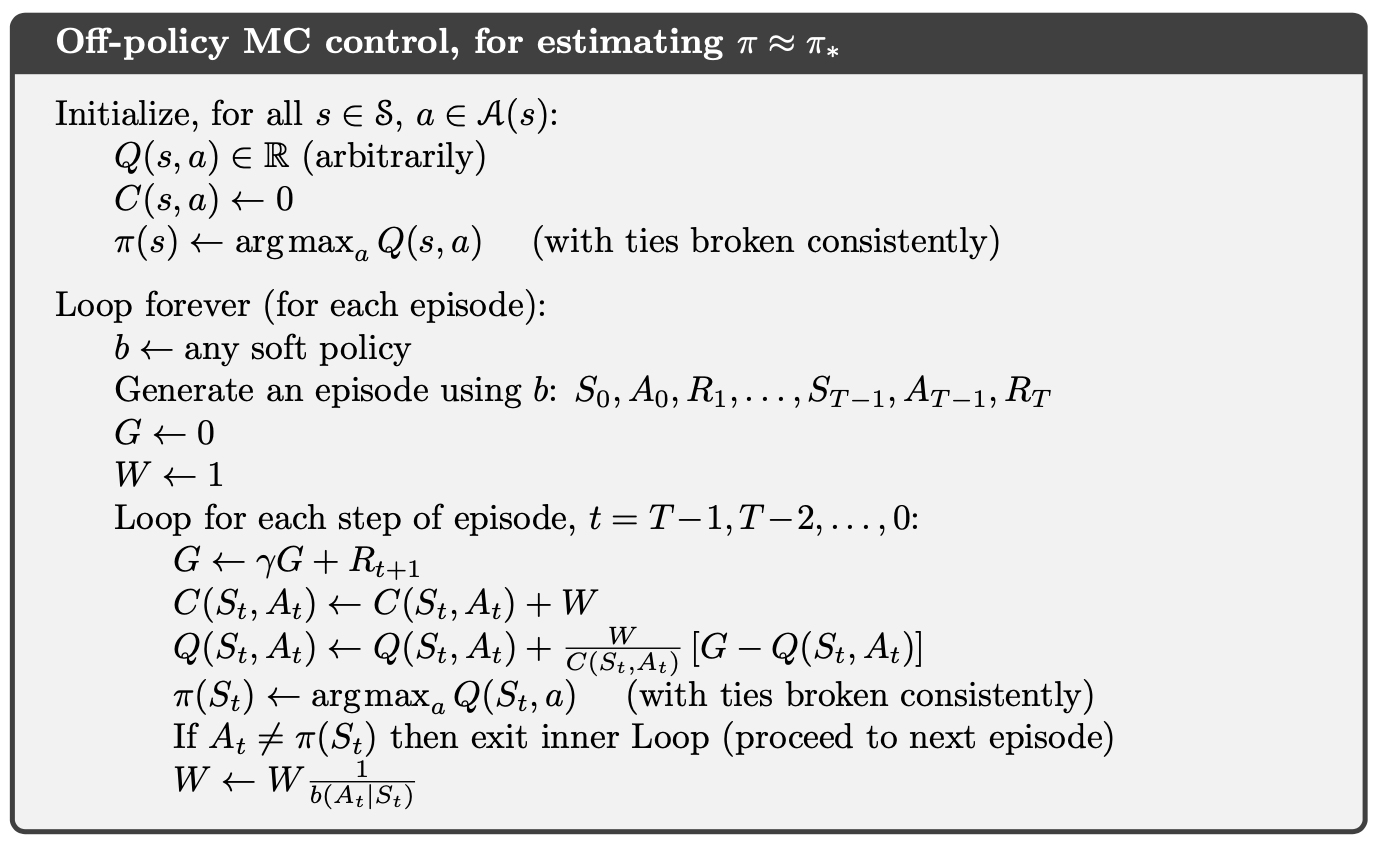
\includegraphics[width=0.6\textwidth]{figures/rl_tabular_methods_offpolicy_MC_control.png}
		\caption{Incremental implementation of Off-policy Monte-Carlo control.}
		\label{fig:rl_tabular_methods_offpolicy_MC_control}
	\end{figure}
	
	Furthermore, to perform the averaging efficiently, we need to keep track of the normalization constant which is the sum of all importance weights for a certain state-action pair. This we will store in $C$. 
	
	In case we use a greedy policy for $\pi$, we can simplify the algorithm further. In the importance weight, $\pi(A_t|S_t)$ is 1 if $A_t$ was the greedy action, otherwise, we have a factor of 0 (which gives $\rho=0$ for all previous actions). If we update our states in a reverse manner, this means that we can stop the loop as soon as we hit a sub-optimal action. 
	
	Note that $W$ can get fairly large for long trajectories, as $b(A|S)$ is always smaller than 1. We need to use weighted importance sampling instead of ordinary as otherwise, the variance is too high. In addition, as only the tails of the episode are updated frequently, we might have an insufficient amount of samples for the states close to the start, which makes the algorithm inefficient.
	
	
\end{itemize}
\subsubsection{On-policy versus Off-policy control}
\label{sec:value_based_tabular_on_off_policy}
\begin{itemize}
	\item After reviewing two alternative ways of learning a policy for a given environment, we can consider what are the advantages and drawbacks of each of the methods
	\item In general, we can note that off-policy is actually a generalization of on-policy because if we set the behavior policy equal to our target policy, i.e. $b=\pi$, then off-policy becomes on-policy
	\item Commonly, on-policy converges faster as it uses the samples from the same policy it updates for. Off-policy can introduce variance by correcting the estimates for the target policy, as e.g. the importance weight can vary a lot if $\pi$ and $b$ are quite different. This can lead to slow convergence.
	\item A benefit of off-policy is however that we can learn from already recorded data, eventually from another source, as only our updates are based on the current policy $\pi$, and not the actual samples as in on-policy. This means that we could use the same data to evaluate multiple policies, which especially helps for limited data/interactions with the environment.
	\item Another point to consider is that off-policy methods allow us to learn the actual greedy policy. This is not possible in the on-policy setting because for guaranteeing the convergence to the correct $q$-values, we need to give every state-action pair a chance greater than zero to be visited. Using an $\epsilon$-soft policy in the on-policy method and greedifying it afterwards can lead to a good approximation, but we also need to keep in mind that we then learn the optimal $\epsilon$-soft policy, and not the strictly the optimal greedy policy. Hence, our final moves might be sub-optimal (remember Cliff-World, Sutton Book Example 6.6, page 132)
\end{itemize}

\subsection{Temporal-Difference Learning}
\begin{itemize}
	\item Combining the ideas of Monte Carlo and Dynamic Programming, we arrive at a different type of methods, called Temporal difference learning. Remember that we can define the value function as a recursive function: $v(s)=\E[R_{t+1}+\gamma v(S_{t+1})|S_t=s]$. We can use this equality as a target instead of $G_t$, leading to the following update rule:
	$$v(s_t)\leftarrow v(s_t)+\alpha\underbrace{\left[R_{t+1}+\gamma v(s_{t+1}) - v(s_t)\right]}_{\text{TD error } \delta_t}$$
	Instead of waiting for a full episode to finish, we can perform this update after \textit{a single action} taken in the environment. This method is called TD(0), and we will see later that this is a special case of TD($\lambda$), or $n$-step TD
	\item TD(0) is a \textit{bootstrapping} method as it uses its own estimates as targets. 
	\item There are two main approaches for learning policies with Temporal Difference, namely \textbf{SARSA} and \textbf{Q-learning}, which we will now discuss in detail. Both learn the $q$-function, but have slightly different update rules.
	
	Note that TD learning can of course also be used for policy evaluation by simply performing the update rule above on samples from the original policy until our value function converges
\end{itemize}
\subsubsection{SARSA}
\begin{itemize}
	\item The update rule of SARSA is as follows:
	$$Q(S_t,A_t)\leftarrow Q(S_t,A_t) + \alpha\left[R_{t+1}+\gamma Q(S_{t+1},A_{t+1})-Q(S_t,A_t)\right]$$
	where $A_{t+1}$ is selected by the policy $\pi$ based on $S_{t+1}$. Note that $Q(S_{t+1},A_{t+1})=0$ for the terminal state.
	\item The method got its name from using $\bm{S}_t$, $\bm{A}_t$, $\bm{R}_{t+1}$, $\bm{S}_{t+1}$, $\bm{A}_{t+1}$ in its update rule.
	\item Note that SARSA is a \textbf{on-policy} method, meaning that it learns the $q$-values of the policy $\pi$ (see Section~\ref{sec:value_based_tabular_on_off_policy} for discussion of benefits and drawbacks)
	\item Instead of just using the next sample to estimate $Q(S_{t+1},A_{t+1})$, we could also take our policy into account as we can calculate the expectation operator over it instead of simply sampling:
	\begin{equation*}
		\begin{split}
			Q(S_t,A_t) & \leftarrow Q(S_t,A_t) + \alpha\left[R_{t+1}+\gamma \E_{\pi}[Q(S_{t+1},A_{t+1})|S_{t+1}]-Q(S_t,A_t)\right]\\
			& \leftarrow Q(S_t,A_t) + \alpha\left[R_{t+1}+\gamma \sum_{a} \pi(a|S_{t+1}) Q(S_{t+1},a)-Q(S_t,A_t)\right]
		\end{split}
	\end{equation*}
	This method is also called \textbf{expected SARSA}
	\item Note that we can perform \textbf{off-policy} control with expected SARSA, where we use a different behavior policy $b$ to sample, but learn the $q$-values of $\pi$. A special case of this is when we choose $\pi$ to be the greedy policy, which leads to the \textbf{Q-learning algorithm}
\end{itemize}

\subsubsection{Q-Learning}
\begin{itemize}
	\item As mentioned before, Q-learning applies a greedy policy in expected SARSA. This simplifies the update rule to:
	$$Q(S_t,A_t)\leftarrow Q(S_t,A_t) + \alpha\left[R_{t+1}+\gamma \max_a  Q(S_{t+1},a)-Q(S_t,A_t)\right]$$
	\item It can be shown that Q-learning converges to the optimal $q_{*}$ under the condition, that the learning rate $\alpha$ goes to zero (but not too fast), and every state-action pair is visited infinite amount of times when we have infinite number of steps.
	\item However, there are also disadvantages of using the greedy policy. Suppose you have multiple actions with the same value $q(s,a)=0$ as ground truth. When learning it, we will have a certain amount of noise on it, so that some are slightly lower and other slightly above 0. When we now take the maximum, $\max_a q(s,a)$, we get a positive value although the GT is zero. Hence, we have a positive bias, to which we also refer to as \textbf{maximization bias}.
	\item This bias can occur when we use a maximum operator in our update step. Hence, it is also the case for SARSA if it uses a $\epsilon$-greedy policy
	\item With infinite number of samples it might become less relevant, but we are usually limited in computational resources/time. Take for example the environment in Figure~\ref{fig:rl_tabular_methods_maximization_bias}. The action of going left has a obviously lower expected reward, but due to the maximization bias, we will have for some actions from $B$ positive rewards (due to a high variance), and hence, we prefer going left. If we limit our number of samples, it is likely that we didn't get a accurate estimate of each of the actions in $B$ yet, and hence, still prefer to go left.
	\begin{figure}[ht!]
		\centering
		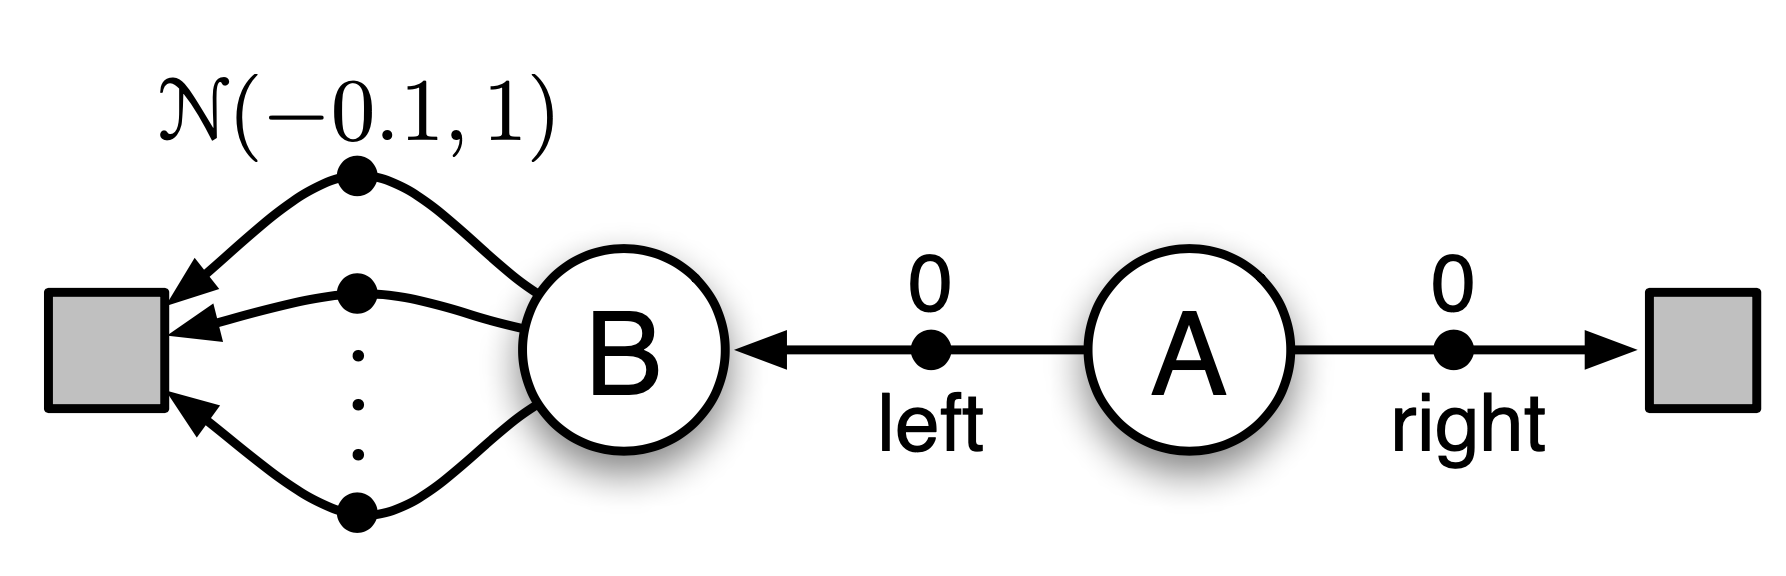
\includegraphics[width=0.3\textwidth]{figures/rl_tabular_methods_maximization_bias.png}
		\caption{Example environment where the maximization bias can lead to a suboptimal policy.}
		\label{fig:rl_tabular_methods_maximization_bias}
	\end{figure}

	\item To overcome this bias, we have to prevent to take the maximum of the estimates as an estimate of the maximum of the true values. So, intuitively, we need to determine the maximizing action from somewhere else than our estimates we are trying to update.
	\item A simple method of doing so is \textbf{Double Q-Learning}. Instead of learning a single $q$-function, we learn two, almost independently. Now, we can update $Q_1$ by using the maximum operator over $Q_2$, and vice versa. By that, we overcome the positive bias as even if $Q_1$ and $Q_2$ are biased themselves, they are positively biased on different actions. 
	\item The general update rule is then:
	\begin{equation*}
		\begin{split}
			\text{Either update }Q_1: \hspace{2mm} Q_1(S_t,A_t) & \leftarrow Q_1(S_t,A_t) + \alpha\left[R_{t+1}+\gamma Q_2\left(S_{t+1},\arg\max_a Q_1(S_{t+1},a)\right)-Q_1(S_t,A_t)\right]\\
			\text{Or update }Q_2: \hspace{2mm} Q_2(S_t,A_t) & \leftarrow Q_2(S_t,A_t) + \alpha\left[R_{t+1}+\gamma Q_1\left(S_{t+1},\arg\max_a Q_2(S_{t+1},a)\right)-Q_2(S_t,A_t)\right]
		\end{split}
	\end{equation*}
	where we randomly assign a sample either to $Q_1$ or $Q_2$ (but not both, because we otherwise get the same bias).
\end{itemize}

\subsubsection{N-step TD learning}
\begin{itemize}
	\item As we will discuss in Section~\ref{sec:value_based_tabular_difference_TD_MC} in detail, both MC and TD have certain advantages and drawbacks. However, we can actually interpolate between these two, which we call $n$-step TD (a generalization of TD(0))
	\item Instead of bootstrapping on the next state, we could use the reward of the $R_{t+2}$ as well, and then bootstrap on $v(S_{t+2})$. This leads to $2$-step TD. It gets obvious, that if we bootstrap always on the terminal state, meaning $\infty$-TD, we arrive at MC as the value of a terminal state is zero. So, we approximate the return $G_{t:t+n}$ for $n$-step TD by:
	$$G_{t:t+n} = R_{t+1}+\gamma R_{t+2} + ... + \gamma^{n-1}R_{t+n} + \gamma^n v_{t+n-1}(S_{t+n})$$
	The update rule is hence:
	$$v_{t+n}(S_t) = v_{t+n-1}(S_t) + \alpha \left[G_{t:t+n}- v_{t+n-1}(S_t)\right]$$
	\item Which $n$ works best, depends on the environment (see Section~\ref{sec:value_based_tabular_difference_TD_MC} for more detailed discussion)
	\item To enable off-policy learning, we would require importance sampling as in MC which can introduce additional variance. However, there is an alternative in $n$-step, namely the $n$-step \textbf{Tree Backup} algorithm
	\item In $n$-step tree backup, we take the next $n$ steps into account, but at each action decision, we also look at all other actions. As visualized in Figure~\ref{fig:rl_tabular_methods_n_step_tree_backup}, we now have multiple leaf nodes. At each of the leafs, we use our estimates.
	\begin{figure}[ht!]
		\centering
		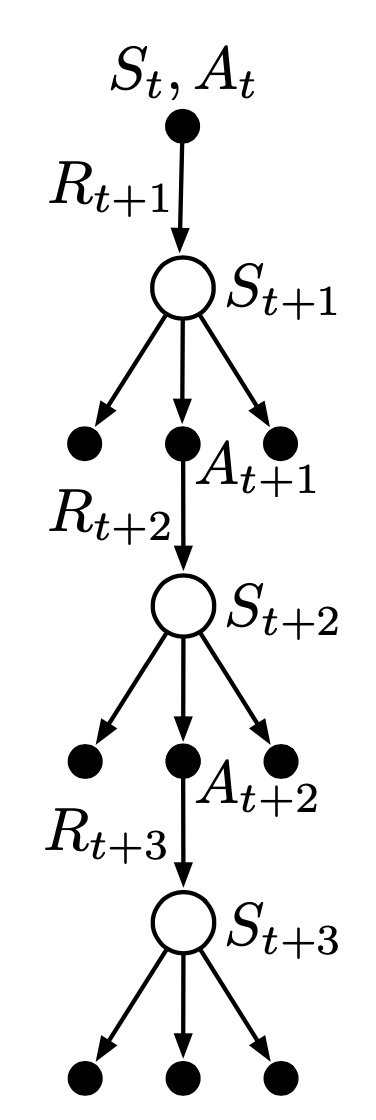
\includegraphics[width=0.1\textwidth]{figures/rl_tabular_methods_n_step_tree_backup.png}
		\caption{3-step tree backup as a backup diagram (see Section~\ref{sec:value_based_tabular_backup_diagram}).}
		\label{fig:rl_tabular_methods_n_step_tree_backup}
	\end{figure}
	\item Even if we sample from a behavior policy $p$, we can re-weight each of the leafs contribution by the target policy $\pi$. For example, at $S_{t+1}$, the leafs are weighted by $\pi(A_1|S_{t+1})$ and $\pi(A_3|S_{t+1})$, while the main sample trajectory gets a factor $\pi(A_2|S_{t+1})$. The next leafs then have $\pi(A_1|S_{t+2})\pi(A_2|S_{t+1})$ etc.
	\item For a 1-step tree backup, we get the same return estimate as for expected SARSA:
	$$G_{t:t+1}=R_{t+1}+\sum_a \pi(a|S_{t+1})Q_t(S_{t+1},a)$$
	If we have $n$ steps, we can calculate our return estimate recursively:
	$$G_{t:t+n}=R_{t+1}+ \gamma\Bigg[\underbrace{\sum_{a\neq A_{t+1}} \pi(a|S_{t+1})Q_{t+n-1}(S_{t+1},a)}_{\text{leaf contributions}} + \underbrace{\pi(A_{t+1}|S_{t+1})G_{t+1:t+n}}_{\text{samples at }t+1}\Bigg]$$
	\item Our behavior policy therefore influences where we generate longer updates, but in expectation (due to the re-weighting), we still get the correct value estimates. Hence, we can use it on off-policy data without needing importance weights ($b$ influences just the depth of certain updates)
\end{itemize}

\subsection{Comparing tabular-based methods}
\begin{itemize}
	\item We have seen now various methods and all take a slightly different approach to Reinforcement Learning
	\item In this section, we compare and review all methods, and put things into perspective
\end{itemize}
\subsubsection{Difference of TD learning and Monte Carlo}
\label{sec:value_based_tabular_difference_TD_MC}
\begin{itemize}
	\item TD can be implemented in an online, fully incremental fashion. In contrast, MC has to wait for the whole episode to finish which can delay learning in applications with very long episodes.
	\item TD learning is stronger influenced by the initial values we give the $v$/$q$-values (and hence by \underline{biased}), which can slow down training. Especially in cases where we try to learn a policy (like Q-learning for TD), we can focus our exploration in the wrong direction for a long time before finding another, optimal case.
	\item In general, MC suffer from \underline{high variance}. This is because $G_t$ is approximated by a single sample, which is often not enough for a sufficient estimate. For example, assume we have a uniform policy over two actions, and an episode is always exactly 10 steps long. Then, the expectation would give each of the $2^{10}=1024$ possibilities a weight factor of $\frac{1}{1024}$ but in MC, we simply pick one of them which clearly is inaccurate.
	\item As usual, there is a trade-off version of both, which is $n$-step TD learning. Which $n$ to choose is highly depending on your environment. For the extreme case of only having a single action to take, MC is clearly preferred because there is no variance in the updates. However, in the case where we can have many different outcomes from the same state, TD learning might be the better option. A common rule of thumb is that we need a lower learning rate for larger $n$ due to the increase of variance
	\item Another interesting difference is that (batch) MC finds the estimates that minimizes the \underline{mean-squared error} on the training set, whereas (batch) TD(0) finds the optimal estimates for a \underline{maximum-likelihood model} of the Markov process. This means that it estimates the transition probability from state $i$ to $j$ as the fraction of observed transitions from $i$ to $j$, and its expected reward is the average of the rewards observed for this transition. Thus, TD learning exploits the Markov property of the environment while MC neglects it. Note that this property can make a big difference if we observe not sufficient data points for each state.
\end{itemize}
\subsubsection{Backup diagrams}
\label{sec:value_based_tabular_backup_diagram}
\begin{itemize}
	\item Another way to visualize the difference between TD and MC is the usage of \textit{backup diagrams}
	\item A backup diagram visualizes a sequence of actions (black dots) and states (white nodes). We always go from a state to a action, which leads us to a next state. One example diagram was already given in Figure~\ref{fig:rl_tabular_methods_n_step_tree_backup}.
	\item Now, consider Figure~\ref{fig:rl_tabular_methods_final_comparison} where we visualize the different extreme cases. TD learning has a shallow update (bootstraps on the next state), while Monte Carlo has infinite depth (i.e. going until the end). The trade-off here is obviously the variance/bias so that $n$-step TD is in between those.
	
	\begin{figure}[ht!]
		\centering
		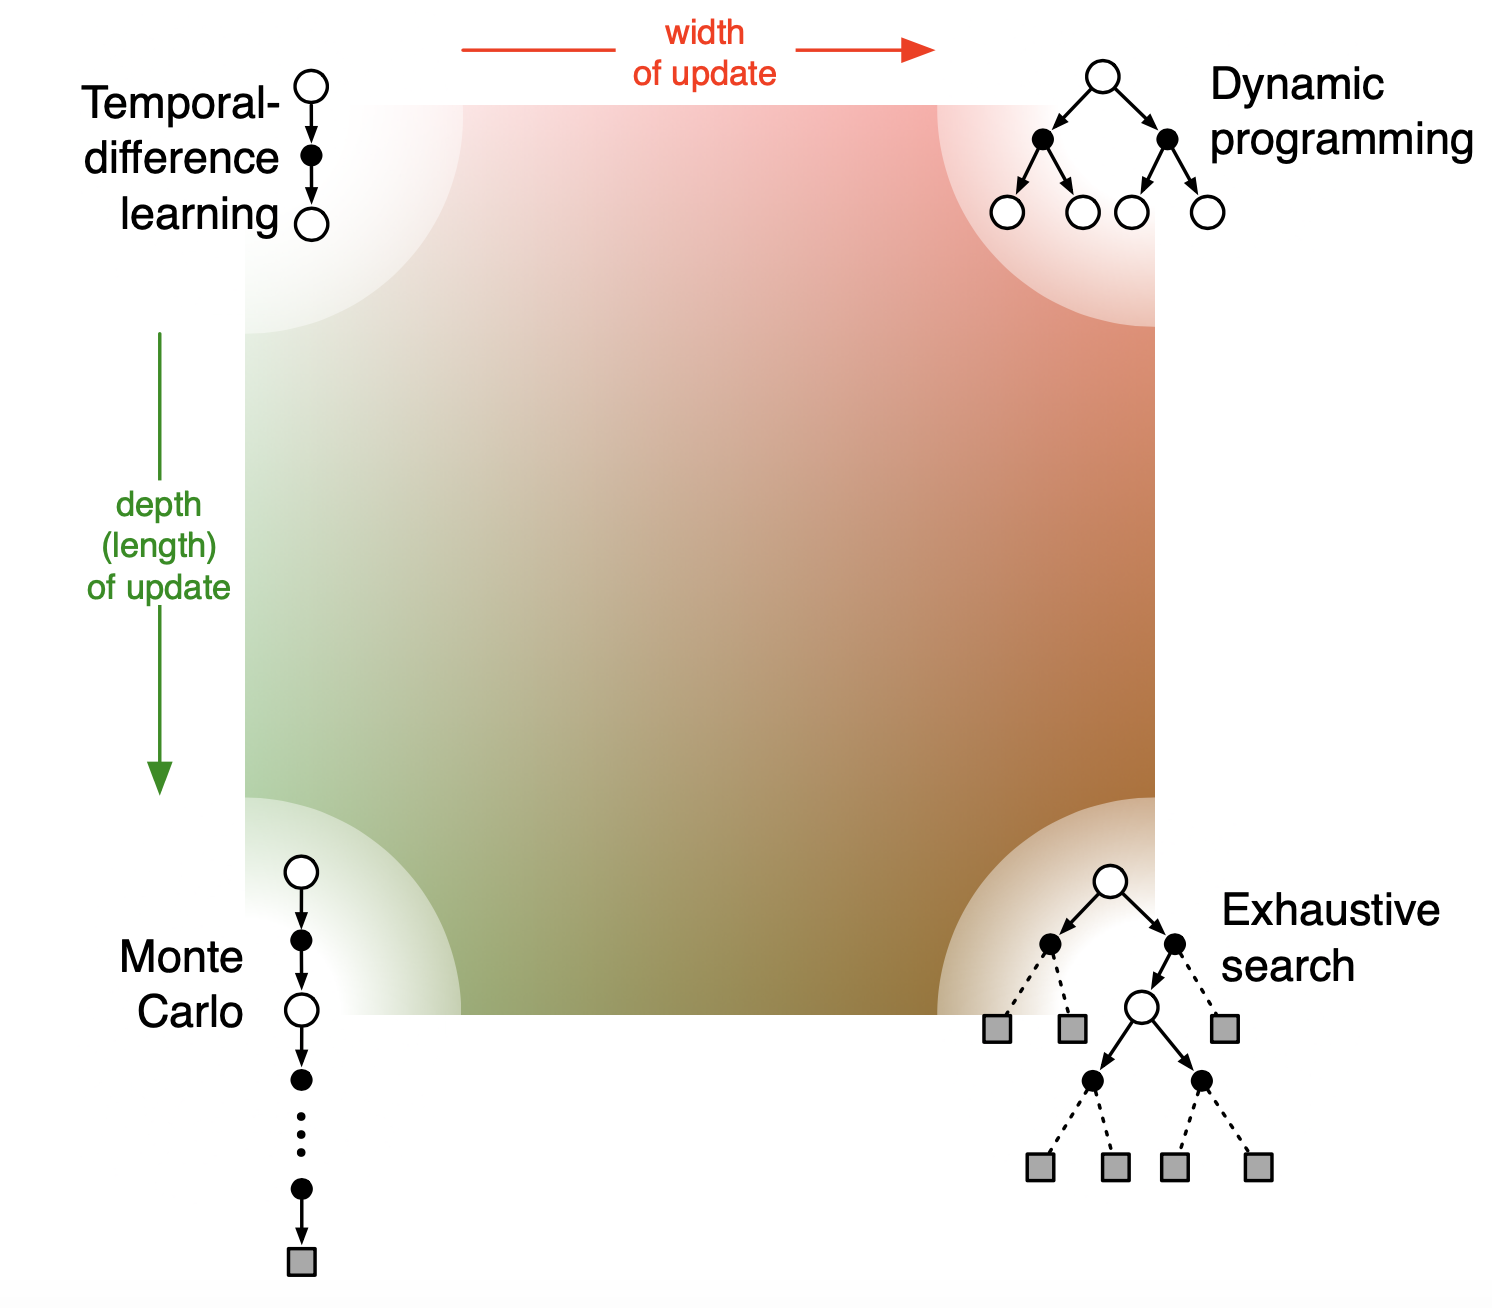
\includegraphics[width=0.4\textwidth]{figures/rl_tabular_methods_final_comparison.png}
		\caption{Putting all methods so far into perspective.}
		\label{fig:rl_tabular_methods_final_comparison}
	\end{figure}
	
	To the right, we get \textit{wider} updates, i.e. move from sampled updates towards expected updates. This means that we consider more actions and states we can end up in. Dynamic programming uses the whole environment dynamics, hence it takes all possible actions and next states into account. In between TD and DP, we can consider expected SARSA or Q-learning as they look at the next actions, but use bootstrapping. 
	
	If we make those methods deeper, we arrive at the $n$-step tree backup algorithm. Making dynamic programming deeper means that we consider \textbf{all} possible outcomes from a given state, which includes possible actions we can get, and possible next states we can end up in. This obviously ends up in a huge, intractable graph for most environments (if we even have given the dynamics) so that it is mostly not feasible to perform.
\end{itemize}
\subsubsection{Limitations so far}
\begin{itemize}
	\item To summarize the tabular-based methods, we want to review their limitations so far.
	\item First of all, as the name indicates, for all the previous methods we store the $q$- and $v$-functions as a table. This is however not always possible. Suppose we have a continuous state space. Then we cannot create a table for that. Alternatively, imagine we want to play an Atari game. Having a screen resolution of $256\times 256$, we would get $256\times 256\times 3\times 256$ different frames (last two factors are channels and 8-bit values of channels) making it infeasible to store. However, it would be also extremely inefficient because similar frames mostly relate to similar actions to take. This leads us to approximate value-based learning methods which we will review in Section~\ref{sec:value_based_approximation}.
	\item Currently, we have to choose the (behavior) policy ourselves with which we explore the environment. Furthermore, if we want to learn an optimal stochastic policy, we also need to set $\epsilon$ in $\epsilon$-soft policies, or the temperature for softmax distributions. But not only for exploration we want randomness, as in partially observable states, we also have uncertainty which we have to take into account. The question arises whether we cannot learn the optimal stochasticity in the algorithm itself, which we will discuss in Section~\ref{sec:policy_learning} and \ref{sec:partially_observable}.
	\item Until we have learned what the effect of our actions are, it takes quite some time for TD and MC to learn. If we want to take sample efficiency into account, we might want to consider model-based approaches as it will be discussed in Section~\ref{sec:model_based}.
\end{itemize}